\subsection{Patron de conception}

Pour le patron de conception, il était évident d'utiliser un modèle en MVC.

Le plus compliqué dans un patron comme celui-ci est d'en faire une implémentation propre avec une réelle séparation des différents composants, tout en gardant une architecture facilement compréhensible.

\subsubsection{L'interface}

Pour l'interface, nous avons choisi de découper chaque fenêtre (à l'exception des pop-ups) dans une nouvelle classe. Ce qui permet 
de pas surcharger la classe de la fenêtre principale, tout en gardant un nombre de classes raisonnable pour notre application.

Nous avons aussi choisi de découper deux grosses parties de la fenêtre principale qui sont la zone de dessin ainsi que les miniatures qui sont des classes à part, héritantes de classes graphiques Qt.

\subsubsection{Le modèle}

Toutes les classes du modèle sont des classes qui héritent de la super-classe QObject car cela permet d'utiliser la technologie des  signaux/slots et ainsi rendre cette partie asynchrone.

Pour les interactions avec le système, nous avons utilisé la classe QProcess afin que ces interactions soient faciles à mettre en place et à observer.

\subsubsection{Le contrôleur}

Le contrôleur est la pièce maîtresse de ce modèle, c'est réellement lui qui fait le lien entre le modèle et l'interface (qui ne discutent JAMAIS directement ensemble).

Il hérite de QObject pour avoir accès aux signaux/slots et n'effectue que très peu d'opérations, il est principalement pour coordonner les actions de l'utilisateur avec les réactions de l'application.

\subsection{Diagramme de classe}
	\begin{center}
		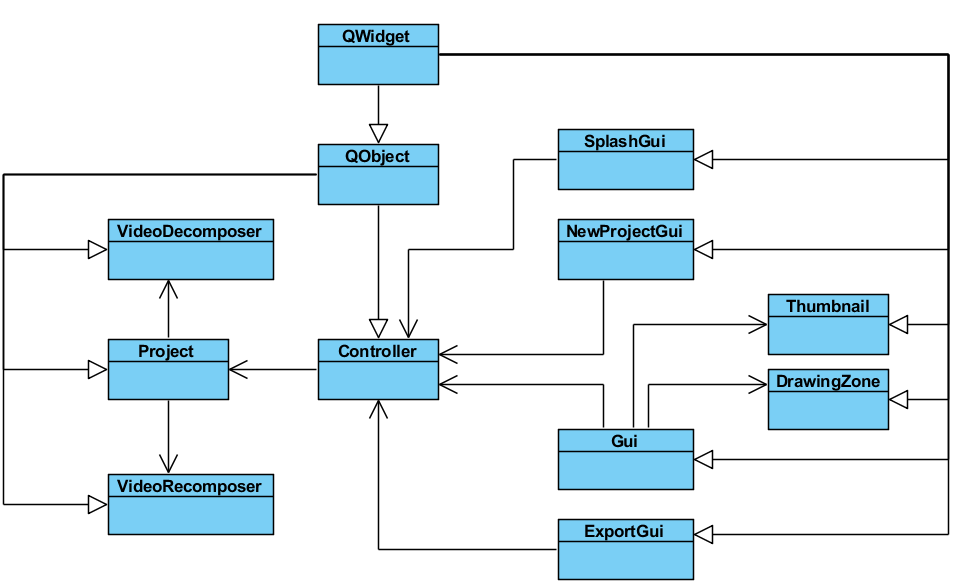
\includegraphics[width=18cm]{./figures/diagramme.png}
	\end{center}
